%% CV - Álvaro López Álvarez
%% Adaptado para: Desarrollador Backend Java Junior/Mid - SOTEC CONSULTING (Grupo Astek)
%%
%% Compilar con: lualatex main_sotec_es.tex
%% (pdflatex suele fallar en instalaciones modernas de MiKTeX con errores de fontawesome5.)

\documentclass[11pt,a4paper,sans]{moderncv}
\moderncvstyle{banking}
\moderncvcolor{blue}

% Fuerza el nombre, apellidos y los títulos de sección al azul de moderncv
% (color1). Por defecto, el estilo banking en lualatex+MiKTeX los deja en
% negro, lo cual desentona con el resto de la paleta azul.
\renewcommand*{\firstnamestyle}[1]{{\fontsize{34}{36}\bfseries\upshape\color{color1}#1}}
\renewcommand*{\lastnamestyle}[1]{{\fontsize{34}{36}\bfseries\upshape\color{color1}#1}}
\renewcommand*{\sectionstyle}[1]{{\sectionfont\color{color1}#1}}

\usepackage[utf8]{inputenc}
\usepackage{needspace}
\usepackage{hyperref}
\hypersetup{
    colorlinks=true,
    linkcolor=blue,
    filecolor=magenta,
    urlcolor=blue,
    pdftitle={Álvaro López Álvarez - CV - SOTEC Consulting},
    pdfpagemode=FullScreen,
}
\usepackage[scale=0.75]{geometry}
\usepackage{import}
\usepackage{eso-pic}

% datos personales
\name{Álvaro}{López Álvarez}
\address{Valencia, España}{}{}
\phone[mobile]{+34 640764553}
\email{alvaro.lopez.dev@gmail.com}
\extrainfo{\href{https://www.linkedin.com/in/alvarolopez-dev}{LinkedIn}, \href{https://github.com/alerone}{GitHub}, \href{https://alerone.github.io/portfolio}{Portfolio}}

% El estilo banking de moderncv (variante de cabecera 3) no conecta \photo -
% se ignora silenciosamente. Se superpone la foto directamente, anclada a la
% esquina de la página para que sea independiente de la cabecera centrada.
\AddToShipoutPictureFG{%
  \ifnum\value{page}=1
    \AtPageUpperLeft{%
      \hspace*{\dimexpr\paperwidth-2.3cm-1.3cm\relax}%
      \raisebox{\dimexpr-1.3cm-2.3cm\relax}{\fboxsep0pt\fboxrule0.6pt\fcolorbox{color1}{white}{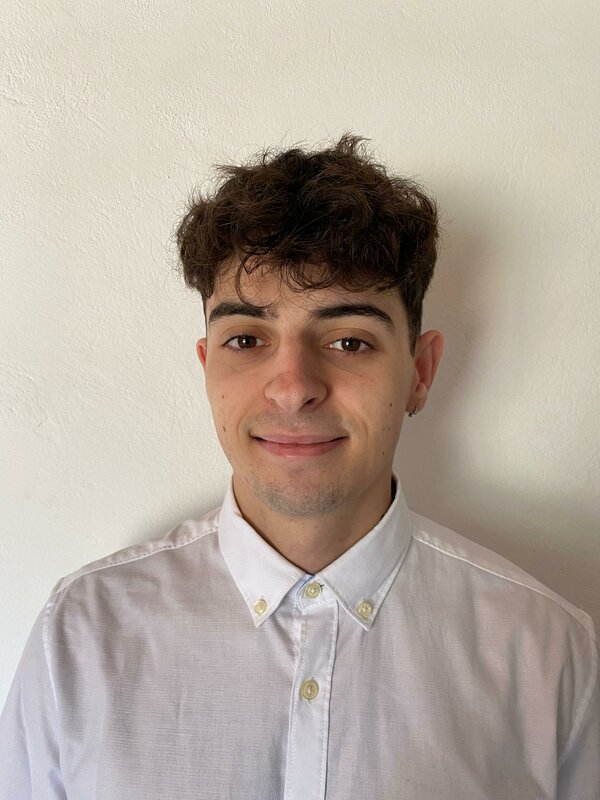
\includegraphics[width=2.3cm]{photo}}}%
    }%
  \fi
}

\begin{document}

\makecvtitle

% ============================================================
%     PERFIL PROFESIONAL
% ============================================================

\vspace{6pt}
\small{Ingeniero de Software Junior con experiencia práctica en backend Java y Spring Boot, construyendo APIs REST respaldadas por persistencia JPA/Hibernate, baterías de pruebas con JUnit y endpoints documentados con OpenAPI. Cómodo trabajando en equipos Scrum/Kanban y flujos de trabajo con control de versiones. Complementa esto con experiencia demostrada en Golang y desarrollo full-stack (React/TypeScript), contenerización con Docker y CI/CD mediante GitHub Actions. Profundiza en Java mediante proyectos autodidactas, incluyendo una plataforma de venta de entradas orientada a eventos con Kafka y un servidor HTTP/1.1 construido desde cero, reflejando un patrón constante de aprendizaje autónomo de nuevas tecnologías.}

% ============================================================
%     COMPETENCIAS CLAVE
% ============================================================

\section{Competencias Clave}
\vspace{1pt}
\begin{itemize}

\item \textbf{Backend Java}: Spring Boot, APIs REST, Hibernate/JPA, documentación OpenAPI/Swagger, JUnit

\item \textbf{Sistemas Distribuidos}: Docker, Apache Kafka, microservicios orientados a eventos

\item \textbf{Práctica Ágil}: equipos Scrum y Kanban, control de versiones con Git, revisiones de código

\item \textbf{CI/CD y Herramientas Cloud-Adjacent}: GitHub Actions, Docker Compose, Testcontainers

\item \textbf{Otros Lenguajes}: Golang, TypeScript/JavaScript (React), Python, Kotlin, SQL

\end{itemize}

% ============================================================
%     EXPERIENCIA PROFESIONAL
% ============================================================

\section{Experiencia Profesional}
\vspace{3pt}
\begin{itemize}

% --- Puesto más reciente ---
\needspace{5\baselineskip}
\item{\cventry{Feb 2026--Jun 2026}{Desarrollador I+D}{Instituto Tecnológico de Informática (ITI)}{Valencia, España}{}{\vspace{1pt}
\begin{itemize}
    \item Implementación de mejoras basadas en LLM para un motor de búsqueda
    \item Desarrollo de un agente multi-paso que convierte preguntas en lenguaje natural en consultas SQL validadas de solo lectura sobre un esquema PostgreSQL, incluyendo validación de seguridad y reintentos ante errores
    \item Aplicación de un diseño agéntico orientado a la seguridad, incluyendo validación de ejecución y reintentos ante errores, dentro de un flujo de trabajo Ágil/Scrum en una plataforma de gobernanza de datos
\end{itemize}}}

\vspace{3pt}

% --- Puesto anterior ---
\needspace{5\baselineskip}
\item{\cventry{Feb 2024--Jun 2024}{Desarrollador Full-Stack (Prácticas)}{Instituto Tecnológico de Informática (ITI)}{Valencia, España}{}{\vspace{1pt}
\begin{itemize}
    \item Desarrollo y mantenimiento de la aplicación corporativa de gestión de personal (Intranet)
    \item Implementación de nuevas funcionalidades de frontend con React y TypeScript, mejorando la usabilidad interna
    \item Contribución al desarrollo backend, garantizando una integración fluida entre servicios mediante flujos de trabajo con Git
\end{itemize}}}

\end{itemize}

% ============================================================
%     PROYECTOS PERSONALES DESTACADOS
% ============================================================

\section{Proyectos Personales Destacados}
\vspace{1pt}
\begin{itemize}

\needspace{3\baselineskip}
\item \textbf{Plataforma de Venta de Entradas con Kafka y Spring Boot}: Microservicios orientados a eventos (reserva, pago, notificación, auditoría) con Spring Boot 3 y Apache Kafka; patrón outbox, colas de mensajes fallidos (dead-letter), procesamiento idempotente y pruebas de integración con Testcontainers.

\needspace{3\baselineskip}
\item \textbf{English Learning API}: API REST en Spring Boot para practicar phrasal verbs y collocations en inglés; entidades JPA, DTOs/mappers, validación con Jakarta, manejo centralizado de errores, ejercicios aleatorios con seguimiento de intentos.

\needspace{3\baselineskip}
\item \textbf{HTTP from TCP (Java)}: Reimplementación en Java de un servidor HTTP/1.1 directamente sobre sockets TCP, construido para profundizar en los fundamentos de Java: I/O, concurrencia mediante executors, pruebas con JUnit.

\end{itemize}

% ============================================================
%     FORMACIÓN ACADÉMICA
% ============================================================

\needspace{9\baselineskip}
\section{Formación Académica}
\vspace{1pt}
\begin{itemize}

\needspace{4\baselineskip}
\item{\cventry{2024--2026}{Máster Universitario en Ingeniería Informática (MUIINF)}{Universitat Politècnica de València (UPV)}{Valencia, España}{}{\vspace{1pt}
En curso (finalización prevista en septiembre de 2026). Temario: sistemas distribuidos, computación de altas prestaciones, ciberseguridad, sistemas empotrados.
}}

\vspace{3pt}

\needspace{4\baselineskip}
\item{\cventry{2020--2024}{Grado en Ingeniería Informática, itinerario de Ingeniería del Software}{Universitat Politècnica de València (UPV)}{Valencia, España}{}{\vspace{1pt}
Nota media: 8,88/10. Trabajo de Fin de Grado (TFG): ``ValenMove -- Aplicación Unificada de Transporte Público'' (calificación 9/10).
}}

\end{itemize}

% ============================================================
%     IDIOMAS
% ============================================================

\section{Idiomas}
\vspace{1pt}
\begin{itemize}
\item Español (nativo), catalán (nativo), inglés (B2, conversación fluida).
\end{itemize}

% ============================================================
%     REFERENCIAS
% ============================================================

\section{Referencias}
\vspace{1pt}
\begin{itemize}
\item{Disponibles a petición.}
\end{itemize}

\end{document}
